% !TEX TS-program = lualatex
%\documentclass[handout]{beamer}
\documentclass{beamer}
\input{../common/misomva}
\newcommand{\misoclasstinytitleslide}{Partially based on material by:  Ulrike von Luxburg, \\[-1em] Gary Miller, Doyle \& Schnell, Daniel Spielman}
\newcommand{\misoclassdate}{}
\usetikzlibrary{graphs}

% TikZ macros for spectral clustering visualizations (defined outside document to avoid beamer issues)
\newcommand{\blob}[3]{\foreach \i in {1,\dots,150} {\draw[#3] (#1 + rand*0.5, #2 + rand*0.5) circle (1.2pt);}}
\newcommand{\ring}[4]{%
    \foreach \i in {1,\dots,250} {%
        \pgfmathsetmacro{\angle}{rand*360}%
        \pgfmathsetmacro{\rad}{#1 + rand*#2}%
        \node[#3, scale=0.6] at (\angle:\rad) {#4};%
    }%
}

\begin{document}
% Topic-specific title slide

\newcommand{\topictitle}{Spectral Clustering: Examples}

\newcommand{\topicsubtitle}{1D Examples and Understanding}

\MakeTopicSlide

%%%%%%%%%%%%%%%%%%%%%%%%%%%%%%%%%%%%%%%%%%%%%%%%%%%%%%%%%%%%

%%%%%%%%%%%%%%%%%%%%%%%%%%%%%%%%%%%%%%%%%%%%%%%%%%%%%%%%%%%%

\begin{frame}
\frametitle{Spectral Clustering: Understanding}
%\textbf{Compactness} vs.\@ \emphcol{Connectivity}}
\textbf{Compactness} vs.\@ \emphcol{Connectivity}\\ \medskip
\pause
% TikZ replacement for compactness (using \blob defined in preamble)
\begin{tikzpicture}[scale=0.45]
    \blob{-2}{-2}{cyan} \blob{-1}{2}{blue!80!black} \blob{1}{0}{brown!70!black}
    \blob{2}{2}{orange} \blob{2}{-1}{green!70!black}
\end{tikzpicture}
% TikZ replacement for connectivity (using \ring defined in preamble)
\begin{tikzpicture}[scale=0.45]
    \ring{1.2}{0.3}{blue}{$\circ$} \ring{2.8}{0.3}{red}{$\times$} \ring{4.5}{0.3}{green!70!black}{$\triangle$}
\end{tikzpicture}
\pause \moves
\questionbox{For which kind of data we can use one vs.\@ the other?}
\pause \moves
\questionbox{Any disadvantages of spectral clustering?}
\end{frame}

%%%%%%%%%%%%%%%%%%%%%%%%%%%%%%%%%%%%%%%%%%%%%%%%%%%%%%%%%%%%
\begin{frame}
\frametitle{Spectral Clustering: 1D Example - Histogram}
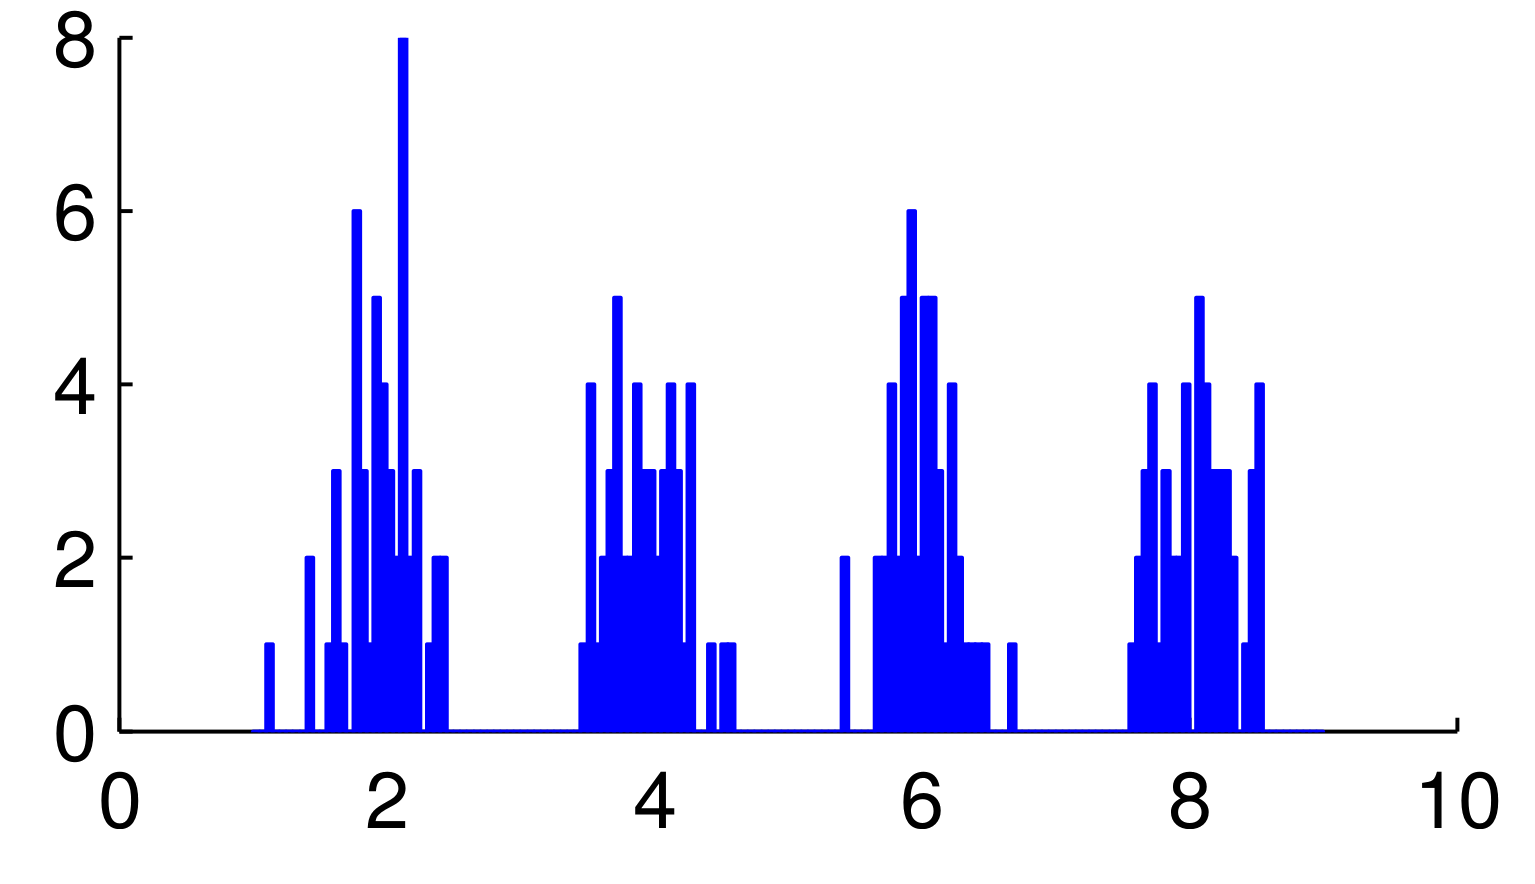
\includegraphics[width=\columnwidth]{../img/luxburgh-example-histogram}
\\
{\scriptsize 
\url{http://www.informatik.uni-hamburg.de/ML/contents/people/luxburg/publications/Luxburg07_tutorial.pdf}
}
\end{frame}
%%%%%%%%%%%%%%%%%%%%%%%%%%%%%%%%%%%%%%%%%%%%%%%%%%%%%%%%%%%%
\begin{frame}
\frametitle{Spectral Clustering: 1D Example - Eigenvectors}
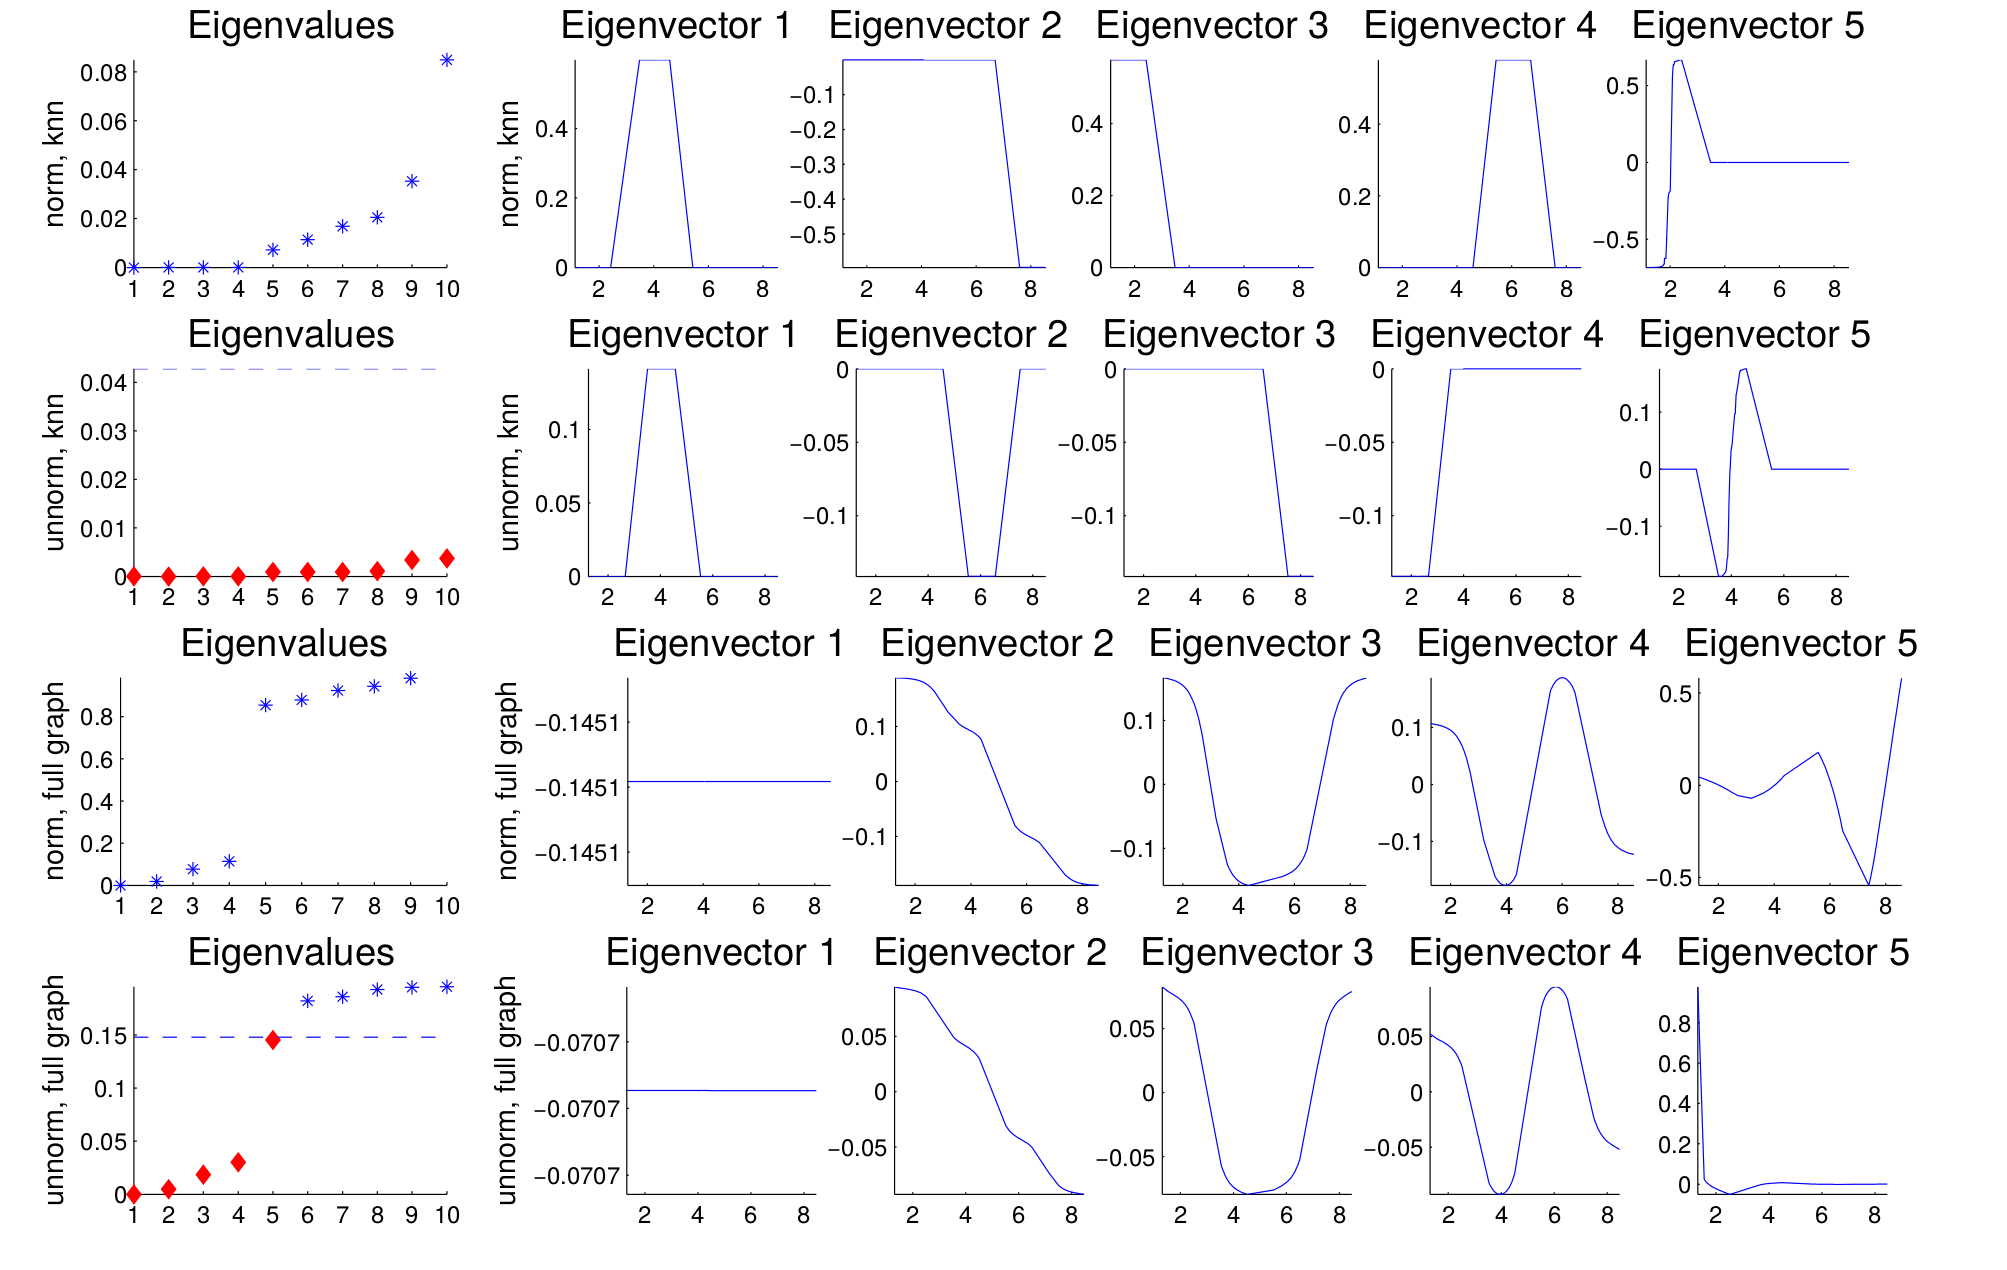
\includegraphics[width=\columnwidth]{../img/luxburgh-example-eigenvectors}
\\
{\tiny Source: von Luxburg (2007)}
\end{frame}
  %%%%%%%%%%%%%%%%%%%%%%%%%%%%%%%%%%%%%%%%%%%%%%%%%%%%%%%%%%%%
\begin{frame}
\frametitle{Spectral Clustering: Bibliography}

\begin{itemize}[<+-| alert@+>]\addtolength{\itemsep}{0.5\baselineskip}
\item \href{https://proceedings.mlr.press/v2/meila02a.html}{\textbf{Meila \& Shi (2001)}} -- A random walks view of spectral segmentation\\
{\small \textit{International Conference on Artificial Intelligence and Statistics}}

\item \grcol{$\bL_{\rm sym}$} \href{https://papers.nips.cc/paper/2001/hash/801272ee79cfde7fa5960571fee36b9b-Abstract.html}{\textbf{Ng, Jordan \& Weiss (2001)}} -- On spectral clustering: Analysis and an algorithm\\
{\small \textit{Neural Information Processing Systems (NIPS)}}

\item \grcol{$\bL_{\rm rm}$} \href{https://ieeexplore.ieee.org/document/868688}{\textbf{Shi \& Malik (2000)}} -- Normalized Cuts and Image Segmentation\\
{\small \textit{IEEE Transactions on Pattern Analysis and Machine Intelligence}, 22(8):888--905}

\item \grcol{Things can go wrong with the relaxation:} \href{https://www.sciencedirect.com/science/article/abs/pii/S0024379506003520}{\textbf{Spielman \& Teng (2007)}} -- Spectral partitioning works: Planar graphs and finite element meshes\\
{\small \textit{Linear Algebra and Its Applications}, 421:284--305}
\end{itemize}

\end{frame}


\MakeLastSlide
\end{document}
